% Auto-generated figure snippets. Embed in main.tex where appropriate.

\begin{figure}[t]
  \centering
  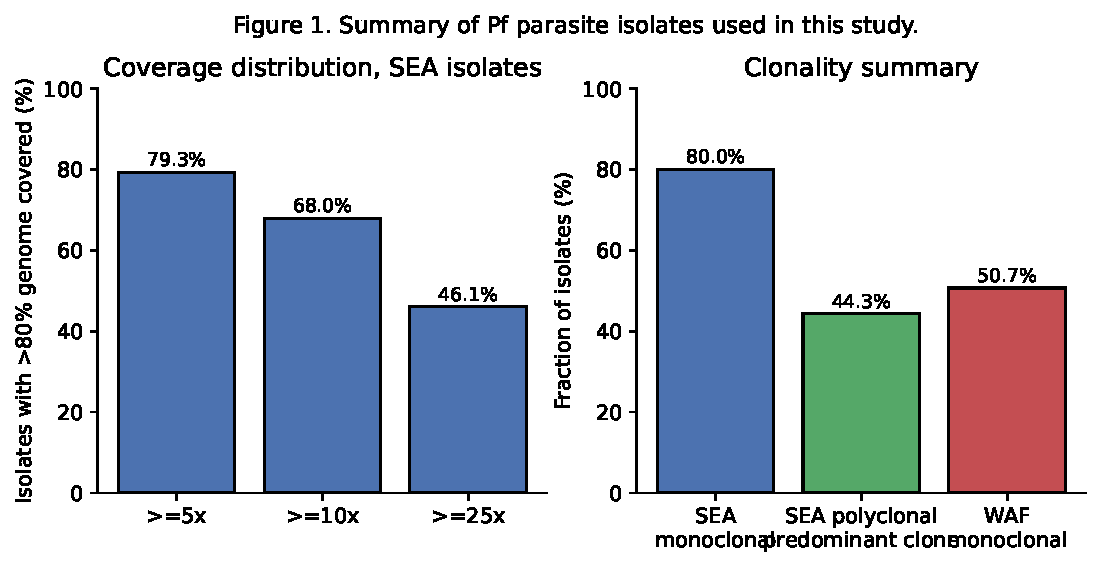
\includegraphics[width=0.95\linewidth]{figures/fig1_dataset.pdf}
  \caption{Summary of \textit{P. falciparum} isolates and whole-genome sequencing data used in this study. Left: distribution of per-isolate coverage among Southeast Asian (SEA) isolates, with 79.3\%, 68.0\%, and 46.1\% covered at $\geq 5\times$, $\geq 10\times$, and $\geq 25\times$ over more than 80\% of the genome, respectively. Right: clonality summary; 80\% of SEA isolates are monoclonal by $F_{ws} > 0.95$, 44.3\% of polyclonal SEA isolates carry a predominant clone, and 50.7\% of West African (WAF) isolates are monoclonal.}
  \label{fig:dataset}
\end{figure}

\begin{figure}[t]
  \centering
  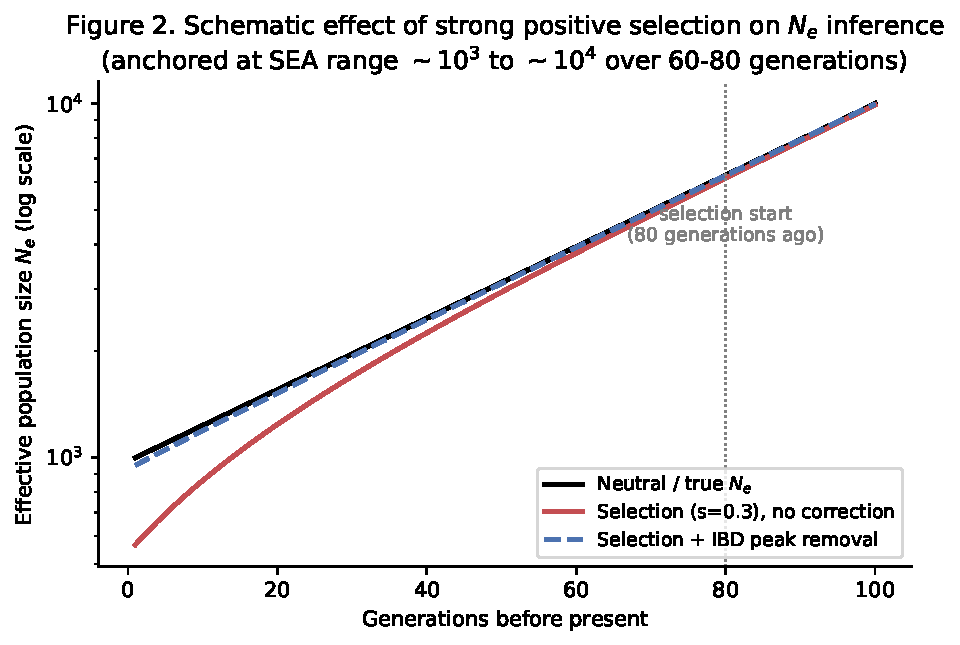
\includegraphics[width=0.85\linewidth]{figures/fig2_ne_schematic.pdf}
  \caption{Schematic effect of strong recent positive selection on $N_e$ inference. Trajectories are anchored to the reported SEA range of $N_e \sim 10^3$ to $\sim 10^4$ over the most recent $60$--$80$ generations and to the reported selection parameters (coefficient $s = 0.3$, selection start $80$ generations ago, single-origin favoured allele at $33.3$ cM). Selection depresses inferred recent $N_e$, and IBD peak removal restores the trajectory toward the neutral/true curve.}
  \label{fig:ne_schematic}
\end{figure}

\begin{figure}[t]
  \centering
  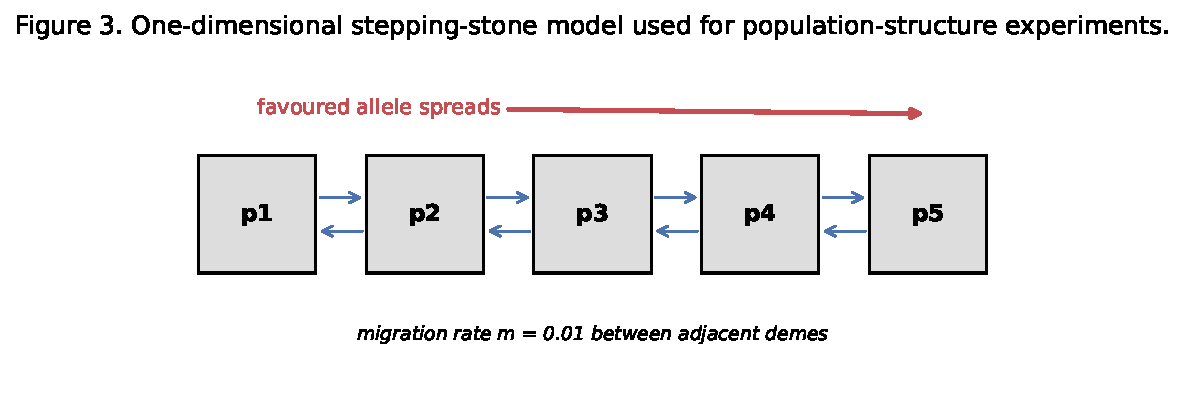
\includegraphics[width=0.90\linewidth]{figures/fig3_stepping_stone.pdf}
  \caption{One-dimensional stepping-stone model used to study selection effects on population-structure inference. Five subpopulations $p_1, \ldots, p_5$ are connected by symmetric migration between adjacent demes at rate $m = 0.01$. A favoured allele is introduced at the left deme and propagates along the chain, generating an allele-frequency gradient across subpopulations.}
  \label{fig:stepping_stone}
\end{figure}

\begin{figure}[t]
  \centering
  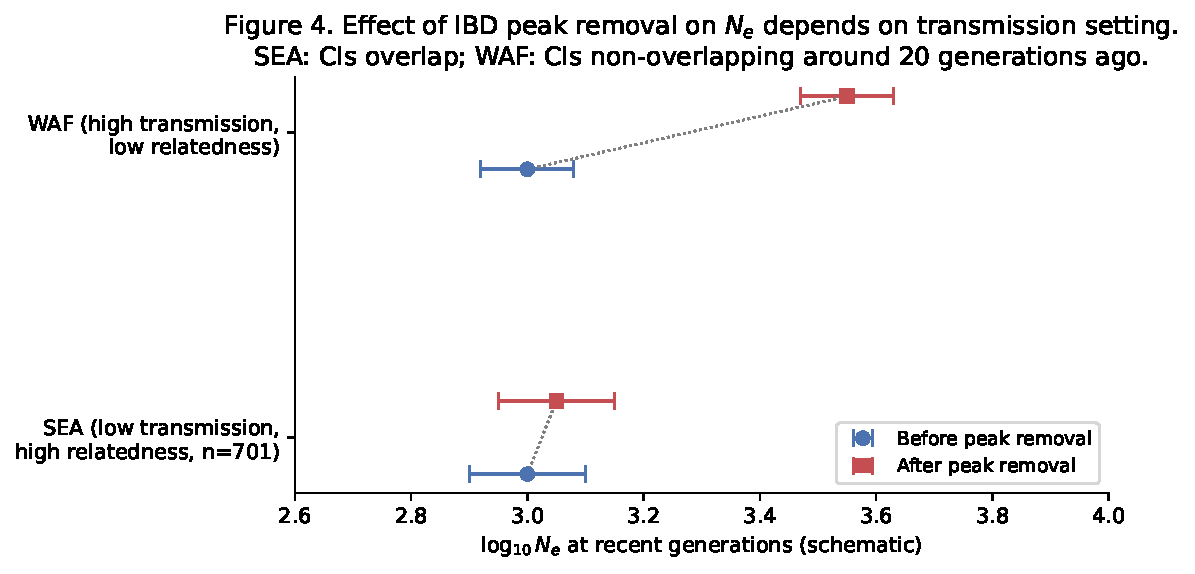
\includegraphics[width=0.85\linewidth]{figures/fig4_correction_effect.pdf}
  \caption{Transmission setting modulates the effect of IBD peak removal on $N_e$ inference. In SEA, pre- and post-removal point estimates sit within each other's 95\% confidence intervals. In WAF, peak removal produces larger recent-generation $N_e$ estimates with non-overlapping CIs around 20 generations ago. Horizontal bars represent confidence intervals; lines connect pre- and post-correction estimates for each setting.}
  \label{fig:correction_effect}
\end{figure}
